% This document is going to serve as a list of definitions for the work that I am doing in
% topological signal processing. This is going to be a living document that I will update it as I
% learn more useful things.

\documentclass[12pt]{article}
\author{Mauricio Montes}

\usepackage{amsmath, graphicx, amssymb}

\title{TDA Introduction and some other concepts}

\begin{document}

\maketitle

\section{Introduction}

This document is for me to keep track of the definitions and ideas I have about topological signal
processing. This will probably get long, so maybe we can chunk it later. I'm not sure if I want to
start all the way with the definition of a topological space. But I think I can start with the ideas
of homology and cohomology. 


\section{Definitions}

\subsection{Topology Preliminaries}

Given a set $X$, a \textit{topology} on $X$ is a set $\mathcal{T} \subset \mathcal{P}(X)$ of subsets
of $X$. The elements of a topology are called \textit{open sets}. To be a topology, certain
requirements must be satisfied. Namely :

\begin{itemize}

  \item $\phi, X \in \mathcal{T}$

  \item For any collection of open sets $\{U_\alpha \}_{\alpha \in I}$, $\bigcup_{\alpha \in I} U_\alpha$

  \item For any finite collection of open sets $\{U_\alpha\}_{\alpha \leq n}$,$\bigcap_{\alpha} U_\alpha$
    
\end{itemize}

\subsection{Simplicial Complexes}

The central objects of simplicial homology are simplicial complexes.

\begin{itemize}

\item A k\textbf{-simplex} is the convex hull of a set of $k+1$ points in some Euclidean space. We can think of a 0-simplex as a
  vertex. A 1-simplex is an edge, a 2-simplex is a triangle, and so on. 

\item Note that a k-simplex has $k+1$ faces, which are the simplices of dimension $k-1$ that are
  contained in it.

\item A \textbf{simplicial complex} is a collection of simplices such that the intersection of any two simplices is either empty or
another simplex.

\item The \textbf{dimension} of a simplicial complex is the maximum dimension of any of the simplices in the complex. 

\end{itemize}

\subsection{Simplicial Homology}

In order to do algebra with simplicial complexes, we need to associate it to algebraic objects that
we can manipulate. This is where the chain complex comes in.

\begin{itemize}

  \item Say $X$ is a $k$-dimensional simplicial complex. The \textit{chain group} $C_k(X,
    \mathbb{R})$ is the vector space (over $\mathbb{R}$) with basis given by the number of
    $k$-simplices in $X$. 

\end{itemize}

\begin{figure}[ht]
  \begin{center}
      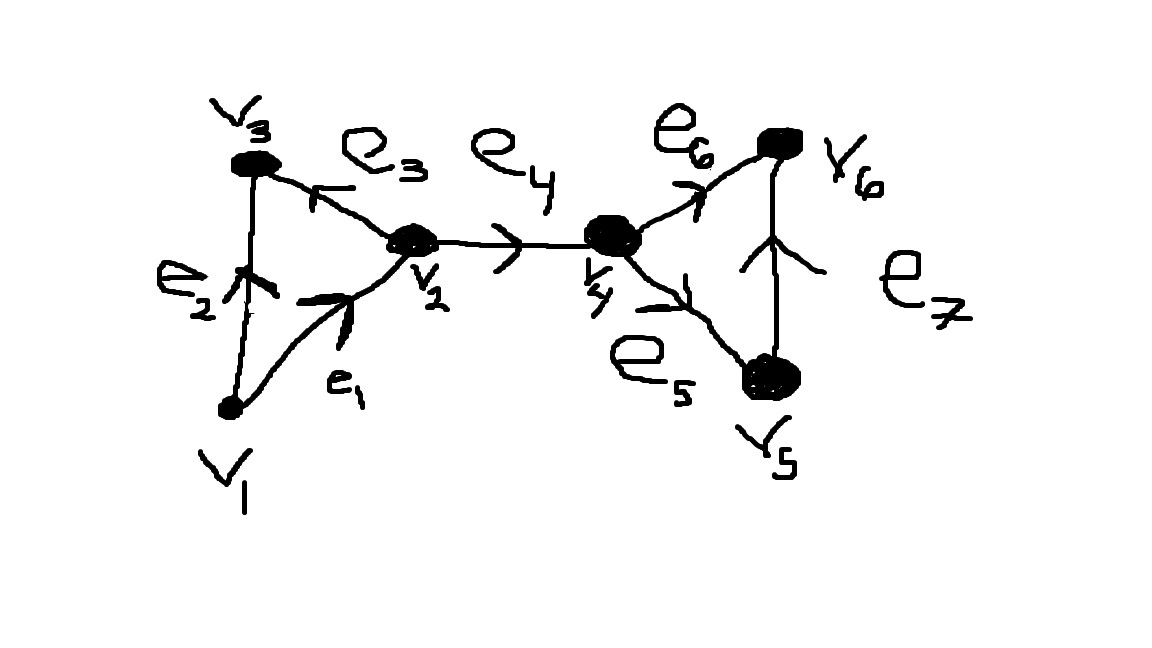
\includegraphics[width=0.5\textwidth]{Simp_Cx.jpg}
  \end{center}
\caption{A simplicial complex, with 6 vertices and 7 edges.}
\end{figure}

Inspecting the image, we see that we have 6 vertices and 7 edges. No higher dimensional simplices. 
We can write down the chain groups associated with this complex: $C_1(X, \mathbb{R}) = \mathbb{R}^6 , C_2(X, \mathbb{R}) = \mathbb{R}^7$


Note that $C_k(X, \mathbb{R}) = 0, k > 2$. For our purposes, we will use $\mathbb{R}$ for our base field for the 
associated vector space and will suppress writing down the associated field for the chain group. Writing 
$C_k(X)$ instead for brevity.

Between chain groups, there exists a map $\delta_{k}: C_k(X) \to C_{k-1}(X)$ given by
\begin{equation}
  \delta_k (v_{i_1}, \ldots v_{i_k}) =  \sum_{j = 0}^{k} (-1)^j (v_{i_1}, \ldots, \hat{v_{i_j}} , \ldots, v_{i_k})
\end{equation}

This is called the \textit{kth chain map}. A set pair of chain groups and chain maps form a \textit{chain complex}.
The associated chain maps have the property that $\delta_{k-1} \circ \delta_{k} = 0$. These chain maps decompose 
into their associated kernel and image maps.

Given a chain complex $C(X)$, we define the \textit{kth homology group} to be $H_k(C) = ker(\delta_k) / Im(\delta_{k+1})$

[INSERT PICTURE OF HIGHLIGHTED ELEMENTS OF THE BOUNDARY MAP HERE]



\subsection{Simplicial Cohomology}

\subsection{Persistent Homology}

\subsection{Hodge Laplacian}

\subsection{Sheaves}

\subsection{Sheaf graph networks}

\subsection{Sheaf Cohomology}

\subsection{Further Directions and Questions}

\begin{itemize}
  \item Is there a theory about probability sheaves? Could one be written down such that
    the maps between sheaves would somehow communicate information about the probability 
    states of network? (Does this question even make sense)

  \item What direct applications could this have towards signal processing? Is there an immediate
    impact besides the answer from Robinson "In theory we can"

  \item What is some nice data that TSP can be used on?

  \item The current methods from TDA and TSP are: Persistent Homology, Bottleneck/Wasserstein distance, 
    0 dimensional sublevel set persistence, 

  \item Homology for lattice configurations?

  \item Homology of dynamical systems

  \item Given a coboundary map $\delta$, we can construct a laplacian matrix associated with a sheaf.

\end{itemize}

\end{document}
